\section{Measurement and Results}
As mentioned above, this experiment has 3 different sets of measurements: 
\begin{itemize}
    \item \textbf{Measurement of Correlation Functions}
    \item \textbf{Violation of Bell’s Inequality}
    \item \textbf{Quantum State Tomography}
\end{itemize}

Thus, this section is also divided into 3 different sections. Each subsection is dedicated to one of the following.

\subsection{Correlation Functions}
In the first part of the experiment, the aim is to measure correlation functions for 2 different cases. In both cases, there are 2 different half-wave plates. One half-wave plate ($HWP_{B}$) is located in the pathway of the photon that goes to Bob, and the other one ($HWP_{A}$) is located in the pathway of the photon that goes to Alice. The angles of the half-wave plates are as follows: 
\begin{itemize}
    \item {Case 1}:
        $\alpha_{HWP_{B}}$ = 0$^\circ$, $\alpha_{HWP_{A}}$ = $i^\circ$ ($i \in$ \{0, 10, 20, 30, 40, 50, 60, 70, 80, 90\})
    \item {Case 2}:
        $\alpha_{HWP_{B}}$ = 22.5$^\circ$, $\alpha_{HWP_{A}}$ = $i^\circ$ ($i \in$ \{0, 10, 20, 30, 40, 50, 60, 70, 80, 90\})
\end{itemize}
For both cases, the angles for the half-wave plates were changed by rotating the half-wave plate. After each configuration, coincidence counts were recorded by the help of a C++ script. Counts for each state and case can be seen below:

% Table for the coincidence counts for the first case
\begin{table}[h!]
    \centering
    \begin{tabular}{|c|c|c|c|c|c|c|c|c|c|c|}
        \hline
        $\alpha_{HWP_{A}}$ & 0$^\circ$ & 10$^\circ$ & 20$^\circ$ & 30$^\circ$ & 40$^\circ$ & 50$^\circ$ & 60$^\circ$ & 70$^\circ$ & 80$^\circ$ & 90$^\circ$ \\
        \hline
        $C_{HH}$ & 251 & 197 & 164 & 76 & 29 & 9 & 28 & 113 & 187 & 216 \\
        $C_{HV}$ & 6 & 18 & 67 & 133 & 196 & 195 & 173 & 111 & 45 & 8 \\
        $C_{VH}$ & 5 & 8 & 67 & 135 & 206 & 232 & 225 & 127 & 56 & 7 \\
        $C_{VV}$ & 205 & 199 & 165 & 73 & 22 & 10 & 36 & 88 & 162 & 234 \\
        \hline
    \end{tabular}
    \caption{Coincidence counts for the first case where $\alpha_{HWP_{B}}$ = 0$^\circ$.}
    \label{tab:coincidence_counts_case1}
\end{table}

\begin{table}[h!]
    \centering
    \begin{tabular}{|c|c|c|c|c|c|c|c|c|c|c|}
        \hline
        $\alpha_{HWP_{A}}$ & 0$^\circ$ & 10$^\circ$ & 20$^\circ$ & 30$^\circ$ & 40$^\circ$ & 50$^\circ$ & 60$^\circ$ & 70$^\circ$ & 80$^\circ$ & 90$^\circ$ \\
        \hline
        $C_{HH}$ & 101 & 161 & 167 & 139 & 108 & 42 & 14 & 25 & 48 & 111 \\
        $C_{HV}$ & 105 & 50 & 26 & 30 & 76 & 154 & 190 & 199 & 155 & 112 \\
        $C_{VH}$ & 86 & 45 & 18 & 42 & 91 & 167 & 186 & 180 & 126 & 82 \\
        $C_{VV}$ & 106 & 183 & 222 & 199 & 157 & 98 & 37 & 21 & 62 & 135 \\
        \hline
    \end{tabular}
    \caption{Coincidence counts for the second case where $\alpha_{HWP_{B}}$ = 22.5$^\circ$.}
    \label{tab:coincidence_counts_case2}
\end{table}

\subsubsection{Calculation of Correlation Functions}
\label{subsubsec:correlation_functions}
To calculate the correlation values, first we need to calculate relative frequencies for each state. Relative frequencies are calculated by dividing the coincidence counts by the total number of counts:
\begin{equation}
    f_{ij} = \frac{C_{ij}}{\sum_{i,j} C_{ij}} \quad (i,j \in \{H, V\})
\end{equation}

After calculating the relative frequencies, we can calculate the correlation values using the following formula with the relative frequencies from \hyperref[tab:coincidence_counts_case1]{Table \ref*{tab:coincidence_counts_case1}} and \hyperref[tab:coincidence_counts_case2]{Table \ref*{tab:coincidence_counts_case2}}:
\begin{equation}
    K_{ij}^{ex} = f_{HH} - f_{HV} - f_{VH} + f_{VV}
    \label{eq:correlation_function}
\end{equation}
with $i, j \in \{H, V\}$. Correlation values for both cases can be seen below:
\begin{table}[h!]
    \centering
    \begin{tabular}{|c|c|c|c|c|c|c|c|c|c|c|}
        \hline
        $\alpha_{HWP_{A}}$ & 0$^\circ$ & 10$^\circ$ & 20$^\circ$ & 30$^\circ$ & 40$^\circ$ & 50$^\circ$ & 60$^\circ$ & 70$^\circ$ & 80$^\circ$ & 90$^\circ$ \\
        \hline
        $Case~1$ & 0.953 & 0.877 & 0.421 & -0.279 & -0.775 & -0.915 & -0.723 & -0.084 & 0.551 & 0.936 \\ 
        $Case~2$ & 0.040 & 0.567 & 0.797 & 0.648  & 0.227  & -0.393 & -0.761 & -0.784 & -0.437 & 0.118 \\
        \hline
    \end{tabular}
    \caption{Calculated correlation values.}
    \label{tab:correlation_values}
\end{table}

The relation between the correlation values and the angles can be visualized by plotting the correlation values against the angles. Since the correlation values are sinusoidal functions, we can fit the correlation values to a sinusoidal function. The fits for both cases can be seen below:
\begin{figure}[h!]
    \centering
    \begin{subfigure}[t]{0.45\textwidth}
        \centering
        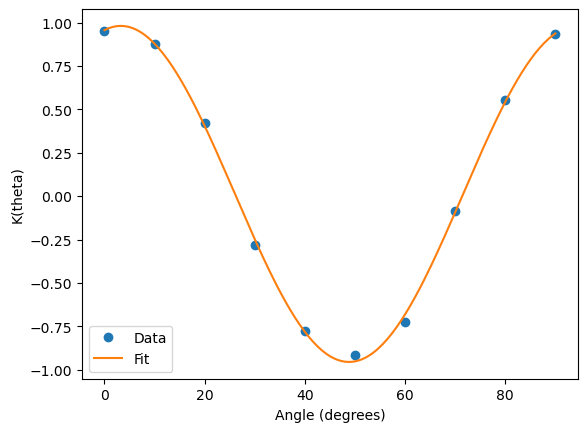
\includegraphics[width=\textwidth]{figures/fit_1.png}
        \caption{Case 1.}
        \label{fig:fit_1}
    \end{subfigure}
    \hfill
    \begin{subfigure}[t]{0.45\textwidth}
        \centering
        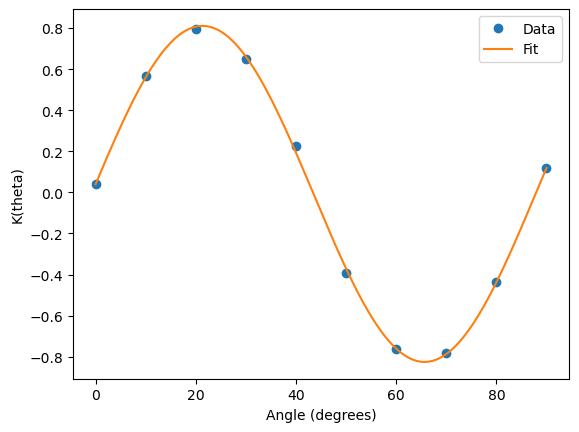
\includegraphics[width=\textwidth]{figures/fit_2.png}
        \caption{Case 2.}
        \label{fig:fit_2}
    \end{subfigure}
    \caption{Correlation values for both cases. 
        $f(\theta) = A \cdot \sin(B \cdot \theta + C) + D$ is used as the fit function.
    }
    \label{fig:fit_comparison}
\end{figure}

\subsubsection{Visibility}
The visibility can be used to parameterize the contrast of measured graphs \cite{manual}. It is defined as the ratio of the difference between the maximum and minimum value of the correlation function to the sum of the maximum and minimum values.
Since a correlation function can be bounded by -1 and 1, the visibility of this function would lead to $\frac{2}{0}$ in a perfect experimental setup. 
To deduce the visibility of the correlation function, we can use a fit function that maps a flat correlation function to 0 and a sinusoidal correlation function to 1.
This can be easily achieved by using the following formula:
\[\mathcal{V} = \frac{\max_{\theta} \tilde{f}(\theta) - \min_{\theta} \tilde{f}(\theta)}{2}\]

This formula will result in a value between 0 and 1, where 0 indicates a flat correlation function and 1 indicates a correlation function varrying between -1 and 1. By using this formula, we can calculate the visibility of the correlation functions for both cases.
{\itshape Case 1} has a visibility of 0.934, while {\itshape Case 2} has a visibility of 0.791.

\subsubsection{Necessity of Two Correlation Functions}
In this experiment, (as any other Bell test experiment) two correlation functions are needed to detect entanglement. Entanglement is a quantum correlation and to be able to detect it, 
we need to detect correlations (measuring correlation functions) in at least two different bases. Just measuring the correlation in one basis is not enough to detect entanglement, since 
correlations in one basis can be explained by classical correlations and local hidden variables\cite{bell,chsh}.  


\subsection{Violation of Bell’s Inequality}
In the second part of the experiment, the aim is to demonstrate the violation of CHSH inequality which is a 
generalization of Bell's theorem\cite{chsh}. As in the first part of the experiment
here we also have one half-wave plate for each party. Unlike the first part, we only have 2 different HWP angles
for each party. The coincidence counts were recorded for each of the 4 possible combinations of the angles.
The angles are as follows:

\begin{table}[h!]
    \centering
    \begin{tabular}{|c|c|c|c|}
        \hline
        \multicolumn{2}{|c|}{Alice} & \multicolumn{2}{c|}{Bob} \\ \hline
        $\alpha$ & $\alpha'$ & $\beta$ & $\beta'$ \\ \hline
        $22.5^\circ$ & $0^\circ$ & $11.25^\circ$ & $-11.25^\circ$ \\ \hline
    \end{tabular}
    \caption{Measurement settings for Alice and Bob.}
    \label{tab:measurement_settings}
\end{table}

The aim of this part is to show that the CHSH inequality is violated. 
The CHSH inequality is defined as follows\cite{chsh}:
\begin{equation}
    |S| \leq 2
\end{equation}
where
\begin{equation}
    S = E(\alpha, \beta) + E(\alpha, \beta') + E(\alpha', \beta) - E(\alpha', \beta')
\end{equation}

The experimental estimation of the correlations are calculated as follows:
\begin{equation}
    E(\alpha, \beta) = \frac{C_{HH}(\alpha,\beta) - C_{HV}(\alpha,\beta') - C_{VH}(\alpha',\beta) + C_{VV}(\alpha',\beta')}{C_{HH}(\alpha,\beta) + C_{HV}(\alpha,\beta') + C_{VH}(\alpha',\beta) + C_{VV}(\alpha',\beta')}
\end{equation}

which is exatly the same as the Equation \ref{eq:correlation_function}.
By using these experimental estimations, we can calculate the CHSH value and show that it is greater than 2.
We assume that the coincidences follow Poisson distribution and the total number of counts
is constant. By using these assumptions, we can calculate the the CHSH value and the error propagation.
The experimental CHSH value is calculated as $2.385 \pm0.015 $ which is greater than the theoretical
maximum value of 2 for classical correlations. This result shows that the CHSH inequality is 
violated and the system is entangled. However, this result is smaller than the 
theoretical maximum value of $2\sqrt{2} \approx 2.828$ for quantum correlations. 
This difference can be explained by the imperfections in the experimental setup.






\subsection{Quantum State Tomography}

In the last part of the experiment, the aim is to do a quantum state tomography for each of the Bell states.
The angles of the waveplates and the correspğonding transformations are given in \hyperref[subsec:measurement_system]{Section \ref*{subsec:measurement_system}}.
As discussed in the \hyperref[subsec:tomography]{Section \ref*{subsec:tomography}}, 
the density matrix of the Bell states can be calculated by using the coincidence counts.
The experimentally constructed density matrices for the Bell states are as follows:

\begin{table}[h!]
    \centering
    \begin{tabular}{|c|}
        \hline
        $|\phi^+\rangle$ \\ \hline
        $\begin{pmatrix}
            0.48 + 0.00i & 0.00 + 0.01i & -0.06 + 0.03i & 0.40 + 0.07i \\
            0.00 - 0.01i & 0.02 + 0.00i & 0.00 + 0.03i & 0.06 - 0.03i \\
            -0.06 - 0.03i & 0.00 - 0.03i & 0.02 + 0.00i & -0.00 - 0.01i \\
            0.40 - 0.07i & 0.06 + 0.03i & -0.00 + 0.01i & 0.48 + 0.00i \\
        \end{pmatrix}$ \\ \hline
        $|\phi^-\rangle$ \\ \hline
        $\begin{pmatrix}
            0.47 + 0.00i & 0.04 - 0.01i & 0.08 - 0.05i & -0.34 - 0.12i \\
            0.04 + 0.01i & 0.03 + 0.00i & 0.01 - 0.02i & -0.08 + 0.05i \\
            0.08 + 0.05i & 0.01 + 0.02i & 0.03 + 0.00i & -0.04 + 0.01i \\
            -0.34 + 0.12i & -0.08 - 0.05i & -0.04 - 0.01i & 0.47 + 0.00i \\
        \end{pmatrix}$ \\ \hline
        $|\psi^+\rangle$ \\ \hline
        $\begin{pmatrix}
            0.03 + 0.00i & 0.05 - 0.04i & 0.05 - 0.05i & 0.01 - 0.04i \\
            0.05 + 0.04i & 0.47 + 0.00i & 0.40 + 0.07i & -0.05 + 0.05i \\
            0.05 + 0.05i & 0.40 - 0.07i & 0.47 + 0.00i & -0.05 + 0.04i \\
            0.01 + 0.04i & -0.05 - 0.05i & -0.05 - 0.04i & 0.03 + 0.00i \\
        \end{pmatrix}$ \\ \hline
        $|\psi^-\rangle$\\ \hline
        $\begin{pmatrix}
            0.06 + 0.00i & 0.10 - 0.03i & -0.15 + 0.07i & 0.02 - 0.01i \\
            0.10 + 0.03i & 0.44 + 0.00i & -0.37 - 0.10i & 0.15 + 0.07i \\
            -0.15 - 0.07i & -0.37 + 0.10i & 0.44 + 0.00i & -0.10 + 0.03i \\
            0.02 + 0.01i & 0.15 - 0.07i & -0.10 - 0.03i & 0.06 + 0.00i \\
        \end{pmatrix}$ \\ \hline
    \end{tabular}
    \caption{Experimentally constructed density matrices of the Bell states.}
    \label{tab:density_matrices}
\end{table}

As discussed in the \hyperref[subsec:tomography]{Section \ref*{subsec:tomography}}, we can calculate
the fidelity, purity and eigenvalues of the density matrices and prove entanglement using the PPT criterion and entanglement witnesses.
The calculated values for the reconstructed Bell states are as follows:
\newpage
\begin{table}[h!]
    \centering
    \begin{tabular}{|c|c|c|c|}
        \hline
        Bell State & Purity & Fidelity & Eigenvalues \\ \hline
        $|\phi^+\rangle$ & 0.80 & 0.88 & (0.89, 0.10, 0.04, -0.04) \\ \hline
        $|\phi^-\rangle$ & 0.71 & 0.80 & (0.85, 0.16, 0.03, -0.04) \\ \hline
        $|\psi^+\rangle$ & 0.78 & 0.87 & (0.89, 0.08, 0.06, -0.03) \\ \hline
        $|\psi^-\rangle$ & 0.78 & 0.80 & (0.90, 0.14, 0.01, -0.05) \\ \hline
    \end{tabular}
    \caption{Purity and fidelity and eigenvalues of the reconstructed Bell states.}
    \label{tab:purity_fidelity}
\end{table}

Reconstructed density matrices have negative eigenvalues, thus they are not positive semidefinite,
which means that they are not physical states. This is also due to the imperfections in the experimental setup.
Another issue is that reconstructed density matrices have different eigenvalues than the theoretical ones.
Any physical pure state has only one non-zero eigenvalue which is equal to 1 and Bell states are pure states.
Thus, the reconstructed density matrices are not pure states.
The purity of the reconstructed density matrices are also less than 1.

\subsubsection{Entanglement Verification of \texorpdfstring{$|\phi^+\rangle$}{|phi+>} with PPT Criterion}
PPT criterion states that if the partial transpose of the density matrix is positive semidefinite,
then the state is separable. Conversely, if the partial transpose has at least one negative eigenvalue,
then the state is an entangled state. The partial transpose of the reconstructed $|\phi^+\rangle$ is as follows:
\begin{equation}
    {|\phi^+\rangle}^{T_B} = \begin{pmatrix}
        0.48 + 0.00i & 0.00 + 0.01i & -0.06 + 0.03i & 0.00 - 0.03i \\
        0.00 - 0.01i & 0.02 + 0.00i & 0.40 - 0.07i & 0.06 + 0.03i \\
        -0.06 - 0.03i & 0.40 + 0.07i & 0.02 + 0.00i & -0.00 - 0.01i \\
        0.00 + 0.03i & 0.06 - 0.03i & -0.00 + 0.01i & 0.48 + 0.00i \\
    \end{pmatrix}
\end{equation}

The eigenvalues of the partial transpose are (-0.39, 0.39, 0.46, 0.54) which means that the state is entangled.

\subsubsection{Entanglement Verification of \texorpdfstring{$|\phi^+\rangle$}{|phi+>} with Entanglement Witnesses}
As discussed in the \hyperref[subsec:tomography]{Section \ref*{subsec:tomography}},
an entanglement witness is a Hermitian operator that has a negative expectation value for entangled states and
entanglement witnesses can be optimized to detect entanglement in a specific state.
The optimized entanglement witness for the $|\phi^+\rangle$ state is as follows:

\begin{equation}
    W = \frac{1}{2} I - |\phi^+\rangle\langle\phi^+|
\end{equation}

The expectation value  of the entanglement witness for the reconstructed
$|\phi^+\rangle$ state is $Tr(W|\phi^+\rangle\langle\phi^+|) = -0.38$ which is less than 0, thus the state is entangled.